\section{ДУ Клеро и Лагранжа}

\begin{Note}[По поводу параграфа (от автора)]
    Если до этого мы рассматривали уравнения, разрешённые относительно производной, то в данном параграфе мы рассмотрим два вида ДУ, которые таковыми не являются.
\end{Note}

\begin{Def}
    Пусть функция 
    \[
        \varphi(t) \in C'(I) \quad and \quad \varphi(t)\; \cancel{\equiv}\; t
    \]
    Тогда ДУ вида 
    \[
        y = x\,y' + \phi(y')
    \] 
    называют диффернциальным уравнением Клеро
\end{Def}

\begin{Note}[Решение ДУ Клеро]
    Дано
    \[
        y = x\,y'(x) + \phi(y'(x))
    \]
    Решение.\\
    Продиференцируем по $x$. Получим
    \[
        \cancel{y'_x(x)} = \cancel{y'_x(x)} + x\,y''_{xx}(x) + \varphi'_t(y')\,y''_{xx}
    \]
    \textcolor{cyan}{Примечание}. Пишем индекс $t$, так как производная от сложной функции.\\
    Таким образом
    \[
        y''(x + \varphi'_t) \equiv 0
    \]
    Рассмотрим 2 случая
    \begin{enumerate}
        \item  $y''_{xx}=0$ Получаем\\
        \begin{align*}
            (y_x')'&\equiv0\\
            y_x' &\equiv C\\
            y&=C\,x + C_1
        \end{align*}
        Требуется проверка, так как мы могли получить лишние решения после \textcolor{red}{диференцирования (это не опечатка?)} (могли появиться в самом начале, когда дифференцировали по $x$)\\
        Проверка. Подставляем ответ в первоначальное решение.\\
        \begin{align*}
            C\,x + C_1 &= C\,x + \varphi(C)\\
            C_1 &= \varphi(C)
        \end{align*}
        \textcolor{red}{Таким образом} общее решение ДУ Клеро выглядит так
        \[
            y = C\,x + \varphi(C)     
        \]
        Нетрудно заметить, что решение выглядит как семейство прямых линий.
                
        \item Рассмотрим второй множитель
        \begin{align*}
            x + \varphi_t'(t) &\equiv 0\\
            x &\equiv - \varphi_t'(t)
        \end{align*}
        Нашли решение относительно $x$ теперь найдём решение относительно $y$.\\
        Пусть $y' = t$, тогда из уравнения условия
        \[
            y = x\,t + \varphi(t)
        \]
        Подставляем $x$ получаем
        \[
            y = -t\,\varphi_t' + \varphi
        \]
        Таким образом, особое решение ДУ Клеро имеет вид
        \[
           L :\: \begin{cases}
                x = - \varphi_t'(t)\\
                y = \varphi - t\,\varphi_t'
            \end{cases}
        \]
        что является уравнением прямой L.
    \end{enumerate}
    \pagebreak

    Графически решение выглядит следующим образом
    \begin{figure}[h]
        \noindent\centering{
            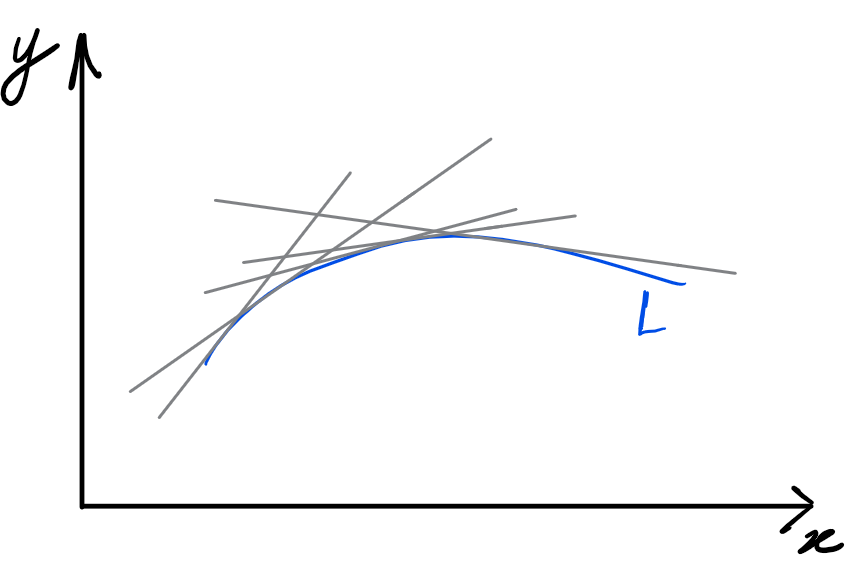
\includegraphics[width=50mm]{2_6_1.png}
            \caption{}
        }
    \end{figure}
\end{Note}

\begin{Note}[О геометрическом смысле ДУ Клеро]
    Ищем кривую $L$, касательные к которой обладают некоторым свойством. Рисунок для условия в конце.

    Уравнение касательной к $L$ в точке $(x,\;y)\in L$\\    
    \[
        Y-y = y'\,(X-x) = y'\,X - x\,y'
    \]
    Уравнение относительно $Y$ в общем виде
    \[
        Y=k\,X+b, \quad \text{где} \quad k=y', \quad b = y - x\,y'
    \]
    Объявим свойство касасательной как $b=\varphi(k)$. Тогда
    \begin{align*}
        y - x\,y' &= \varphi(y')\\
        y &= x\,y' + \varphi(y')
    \end{align*}
    Таким образом, мы получили уравнение Клеро.
    \begin{figure}[bh]
        \noindent\centering{
            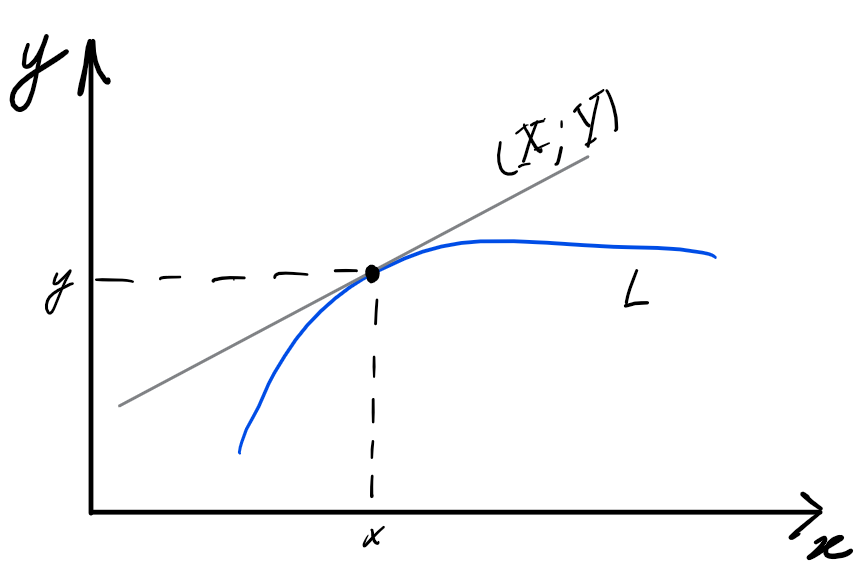
\includegraphics[width=75mm]{2_6_2.png}
            \caption{}
        }
    \end{figure}
\end{Note}

\begin{Def}
    Пусть есть функции
    \[
        (\varphi(t),\; \psi(t)) \in C'(I) \quad \varphi(t)\; \cancel{\equiv}\; t \text{ (функция нелинейна)}
    \]
    Тогда уравнение вида 
    \[
        y=x\,\varphi(y')+\psi(y')
    \] 
    называют ДУ Лагранжа.\\  
    \textcolor{cyan}{Замечание 1}. Уравнение похоже на Клеро, но тут кривая связана с нормалями.\\
    \textcolor{cyan}{Замечание 2}. \textcolor{red}{Уравнение Лагранжа общий случай уравнения Клеро.}
\end{Def}

\begin{Note}[Как решать]
    Дано
    \[
        y=x\,\varphi(y')+\psi(y')
    \]
    Решение.\\
    Введём следующую параметризацию
    \[
        \begin{cases}
            x = x(t)\\
            y = y(t)
        \end{cases}
    \]
    Тогда формуле параметрически заданной функции получаем
    \[
        y'_x=\frac{y'_t}{x'_t}=t \qquad \Rightarrow \qquad y'_t=t\,x'_t
    \]
    Так как $y'_x$ и $y'$ одно и тоже, получаем из условия
    \[
        y = x\,\varphi(t) + \psi(t)
    \]
    Продиференцируем по $t$ Получим
    \[
        y'_t = x'_t\,\varphi + x\,\varphi'_t + \psi'_t
    \]
    Помним, что $y'_t = t \, x_t'$. С учётом этого уравнение выше приобретает вид
    \begin{align*}
        x'_t\,\varphi + x\,\varphi'_t + \psi'_t = t \, x_t'\\
        x'_t\,(\varphi - t) + x\,\varphi'_t = -\psi'_t
    \end{align*}
    Таким образом получили линейное ДУ 1-го порядка в приведённой форме. Решение (через метод Лагранжа)
    \begin{align*}
        x'_t + \frac{\varphi\,'_t}{\varphi-t}\,x &= \frac{\psi'_t}{\varphi-t}\\
        x_0' + \frac{\varphi'_t}{\varphi-t}\,x_0 &= 0\\
        x_0' = \frac{\varphi'_t}{t - \varphi}\,x_0\\
        \frac{dx_0}{x_0} = \frac{\varphi'_t\, dt}{t - \varphi}
    \end{align*}
    Интегрируем и получаем решение для однородного ДУ затем находим ответ для неодродного уравнения ($x_1$). Таким образом мы нашли 
    \[
        x=x_1(t)+C\,x_0(t)
    \]
    Подставляем значение $x$ в $y'_t=t\,x'_t$ или $y = x\,\varphi(t) + \psi(t)$ \textcolor{red}{(оба варинта справедливы?)}. Получаем окончательный ответ.\\
    Таким образом, общий интеграл ДУ Лагранжа
    \[
        \begin{cases}
            x=x_1(t)+C\,x_0(t)\\
            y=y_1(t)+C\,y_0(t)
        \end{cases}
    \]
    Замечание. Нужно проверить\\
    \[
        \frac{y'_t}{x'_t}=t
    \]
    особое решение, когда $\varphi(t)-t=0$\\
\end{Note}



